% Modified 31 Oct 2005:  Conditioning fallacy alluded to.
% This chapter has been modified on 6-4-05.
% There are two \choice
\pagestyle{headings}
\chapter{Discrete Random Variables} \label{chp 3}
\thispagestyle{fancy}

\subsection*{Introduction: Payout on Tails}
Consider a gambling game in which a coin is repeatedly flipped until the first tail appears. The payout is determined by the number of heads that occur before this first tail. If $n$ heads occurred then the player receives $\$\,n$.

\eqns{T &\rightarrow \$\,0 \\ HT &\rightarrow \$\,1 \\ HHT &\rightarrow \$\,2\\ HHHT &\rightarrow \$\,3 \\ & \vdots}
\par
How much should a rational player be willing to pay in advance to play this game? Certainly if you could play for free you would, and it's not hard to convince yourself that paying $50$\,\textcent\ to play is a rational decision. Why? The first flip is heads with probability $\frac{1}{2}$, and in this case the payout will be at least $\$\,1$, possibly much more. Hence the two events `leaving with $50$\,\textcent\ less than you came with' and `leaving with at least $50$\,\textcent\ more than you came with' are equally likely.
\par
We would like to be more precise, and determine exactly where the break even point lies. Is it still rational to play the game for $\$\,0.75$? For $\$\,1$? For $\$\,2$? At what point does the game shift from favouring the player to favouring the house?
\par
The player's payout in this game is an example of a \emph{random variable}, which is a real number whose value is determined by the outcome of an experiment that involves some randomness or element of chance. Random variables are the central object of study in probability \& statistics, and they'll stick around for the rest of the course.
\newpage

\section{Discrete Probability Distributions} \label{sec 3.1}

\begin{defn}\index{Random Variable}\label{RandomVariableDef} A random variable is a function from a sample space $\Omega$ to $\mathbb{R}$. 
\par
\noindent If all values in the range of this function can be listed one-by-one (whether that list is finite or infinite), the random variable is called discrete. In this section, we'll deal only with discrete random variables.
\end{defn}
\par
Recall that a sample space represents the set of all outcomes of some experiment, so a random variable associates a real number with each possible outcome. In other words, a random variable is simply a variable whose value depends on the outcome of an experiment.
\par
Random variables are typically denoted using capital letters at the end of the alphabet, such as $X$, $Y$, or $Z$, and the probability the random variable $X$ takes the value $a$ is denoted $P(X = a)$. This probability can be determined by computing the probability of an event in the sample space on which $X$ was defined.

\begin{examp} Let $X$ denote the outcome of single die roll. Then $X$ is a random variable defined on the sample space $\Omega = \{1,2,3,4,5,6\}$.
\par
\noindent Not surprisingly, $P(X = 1) = \frac{1}{6}$, $P(X = 2) = \frac{1}{6}$, and so on. We could also ask for $P(X > 4)$, and again you should not be surprised that $P(X > 4) = \frac{2}{6}$.
\end{examp}

\par
Notice that any equation or inequality involving a random variable determines some subset of outcomes (an event) in $\Omega$, and so the probability of the equation or inequality holding is the probability that this event occurs.
\par
In fact, for any event $E \subseteq \Omega$, we can define an indicator variable $I_{E}$, which takes the value $1$ if $E$ occurs and $0$ if $E^c$ occurs. 

\begin{examp}Consider rolling a pair of dice and define $S =$ `a sum of seven was rolled', find $P(I_S = 1)$ and $P(I_S = 0)$.
\par
\noindent By definition of $I_S$, we have $P(I_s = 1) = P(S)$ and $P(I_s = 0) = P(S^c)$. From the table constructed in Section \ref{sec 1.1}, $P(I_s = 1) = \frac{6}{36}$ and $P(I_s = 0) = \frac{30}{36}$.
\end{examp}

\begin{examp} Let $X$ denote the number of hearts in three draws, with replacement, from a shuffled deck. What is $P(X > 1)$?
\par
\noindent We are asking for the probability that more than one heart is drawn in three draws, with replacement. Using the law of total probability or a tree diagram,
\eqnsgap{P(X > 1) = \frac{1}{64}+ \frac{3}{64}+ \frac{3}{64}+ \frac{3}{64} = \frac{10}{64}\simeq 0.156.}
\end{examp}
\par

\begin{rmk} Note that random variables must take real number values. If we let $X$ denote the number of heads in a single flip of a coin, then $X$ is a random variable, but if we let $X$ denote the outcome (Heads or Tails) of a single flip of a coin, then $X$ is not a random variable.
\end{rmk}

We can summarize a random variable by listing every possible value it can take, and writing the probability it takes each of those values. To do so is to give the probability distribution of the random variable $X$. 

\begin{defn}\index{Random Variable! distribution of}
The probability distribution of a random variable $X$ associates to every possible value of $X$ the probability that it occurs.
\end{defn}

Often we'll drop the word probability from the definition and refer simply to `the distribution of $X$'. The simplest way to present the distribution of a discrete random variable is through a table.

\begin{examp} Suppose that a fair coin is flipped twice, and let $X$ be the number of heads observed. Write the distribution of $X$ using a table.
\par
\noindent
Let's take $\Omega = \{HH, HT, TH, TT\}$ for our sample space, and since the coin is fair, each of the four outcomes should be equally likely. In two of the four outcomes, one head is observed, in one outcome no heads are observed, and in one outcome two heads are observed.
\renewcommand*{\arraystretch}{1.35}
\begin{center}
\begin{tabular}{c|c}
$x$ & $P(X = x)$ \\
\hline
$0$ & $\frac{1}{4}$ \\
$1$ & $\frac{2}{4}$ \\
$2$ & $\frac{1}{4}$ \\
\end{tabular}
\end{center}
\renewcommand*{\arraystretch}{1}
\end{examp}

\rmk Notice that capital letters are used to denote random variables while lower case letters are used to denoted possible values that random variables may take.

\subsection*{Probability Mass Functions}
\par
If we define a function $f_X: \mathbb{R} \to \mathbb{R}$ by assigning to each possible value of $X$ the probability it occurs, the result is called the probability mass function of $X$. Note that if $x$ is any value which $X$ never takes, then we define $f_X(x) = 0$.

\begin{defn}\index{Probability Mass Function}
The probability mass function (abbreviated pmf) $f_X$ for the random variable $X$ is defined by $f_X(x) = P(X = x)$.
\end{defn}

\begin{examp} Let $Y$ denote the sum of the to numbers showing when a pair of dice is rolled. Graph the probability mass function $f_Y$.
\par
\noindent
From the table in Section \ref{sec 1.1}, we know $Y$ can take any integer value between $2$ and $12$ inclusive. We can also see $P(Y = 2) = \frac{1}{36}$, $P(Y = 3) = \frac{2}{36}$, $P(Y = 4) = \frac{3}{36}$, and so on. Plotting these values, we obtain the probability mass function $f_Y$ shown below.
\begin{center}
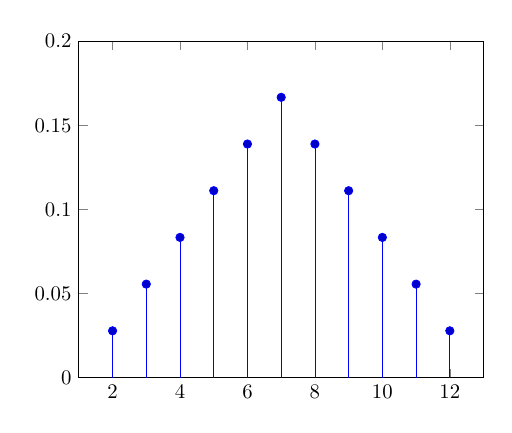
\begin{tikzpicture}[scale = 0.75]
\begin{axis} [ymin = 0, ymax = 0.2,
		y tick label style={
        /pgf/number format/.cd,
            fixed,
            precision=2,
        /tikz/.cd
    }]
\addplot+[ycomb] plot coordinates {(2,1/36) (3,2/36) (4,3/36) (5,4/36) (6,5/36) (7,6/36) (8,5/36) (9,4/36)(10,3/36) (11,2/36) (12,1/36)}; 
\end{axis} 
\end{tikzpicture}
\end{center}
\end{examp} 
\par
The vertical lines under each point are not technically part of the graph of $f_Y$, but are often drawn to make the graph easier to construct and interpret. One can also think about the pmf as a bar graph displaying the number of outcomes for each possible value of $X$ when we take a very large number of samples.
\par
\begin{prop}\label{pmfproperties} Suppose that $X$ is a discrete random variable which takes values in the set $A = \{x_1, x_2, x_3, \, ...\}$. Then the probability mass function $f_X$ satisfies the following properties.
\vspace{-0.5em}
\begin{enumerate}[(i)]
\item $f_X(x) \geq 0$ for all $x \in \mathbb{R}$.
\item $f_X(x) = 0$ for all $x \not\in A$.
\item $\sum_{x \in A} f_X(x) = 1$.
\end{enumerate}
\end{prop}
\par
In fact, these properties completely characterize the class of probability mass functions for discrete random variables. In other words, if $f$ is a function with these three properties, then it is the pmf of a discrete random variable.

\begin{example}
Find the value of $k$ so that the function $h$ below is a pmf.
\renewcommand*{\arraystretch}{1.35}
\eqns{h(x) = \left\{
\begin{array}{cl}
      \left(\frac{1}{3k}\right)^x & \text{ if \ } x = 1, 2, 3, ... \\
      0 & \text{otherwise} \\ \end{array} 
\right.}
\renewcommand*{\arraystretch}{1}
\par
\noindent As long as $k$ is positive, $h$ will satisfy properties $(i)$ and $(ii)$ above. The last property allows us to determine $k$ uniquely.
\eqns{\sum_{x \in A} h(x) =  \sum_{x = 1}^{\infty} \left(\frac{1}{3k}\right)^x = \frac{1}{3k} +  \left(\frac{1}{3k}\right)^2 +  \left(\frac{1}{3k}\right)^3 + ... = \frac{\frac{1}{3k}}{1-\frac{1}{3k}} = \frac{1}{3k - 1} }
\par
\noindent The geometric series sum formulas was used to evaluate the infinite sum. Setting the last expression equal to 1 gives $3k - 1 = 1$, and hence $k = \frac{2}{3}$. Using this value of $k$ gives the function $h$ below, which we can graph as a pmf.
\renewcommand*{\arraystretch}{1.35}
\eqns{h(x) = \left\{
\begin{array}{cl}
      \left(\frac{1}{2}\right)^x & \text{ if \ } x = 1, 2, 3, ... \\
      0 & \text{otherwise} \\ \end{array} 
\right.}
\par
\noindent Of course, only the first few values can be shown, since the graph continues off to the right indefinitely.
\renewcommand*{\arraystretch}{1}
\begin{center}
\begin{tikzpicture}[scale = 0.75]
\begin{axis}[ymin = 0, ymax = 0.3,
		y tick label style={
        /pgf/number format/.cd,
            fixed,
            precision=2,
        /tikz/.cd
    }]
\addplot+[ycomb] plot coordinates {(1,1/2) (2,1/4) (3,1/8) (4,1/16) (5,1/32) (6,1/64) (7,1/128) (8,1/256)}; 
\end{axis} 
\end{tikzpicture}
\end{center}
\end{example}

\subsection*{Functions of a Discrete Random Variable}
\par
If $X$ is a discrete random variable, and $g: \mathbb{R} \to \mathbb{R}$ is any function, then $Y = g(X)$ is also a discrete random variable. Its value is completely determined by $X$.

\begin{examp}\label{FunctionRVEx}
Let $X$ be the random variable whose pmf is given below, and let $Y = 1 + X^2$. Find the pmf of $Y$.
\begin{center}
\begin{tikzpicture}[scale = 0.6]
\begin{axis}[ymin = 0, ymax = 0.4,
		y tick label style={
        /pgf/number format/.cd,
            fixed,
            precision=2,
        /tikz/.cd
    }]
\addplot+[ycomb] plot coordinates {(-1,2/10) (0,1/10) (1,2/10) (2,2/10) (3,3/10)}; 
\end{axis} 
\end{tikzpicture}
\end{center}
\par
\noindent We need to calculate $Y$ for each possible value of $X$, and sum up the probabilities when appropriate. In this case, note that there are two values of $X$ which result correspond to $Y = 2$, so $f_{Y}(2) = f_X(-1) + f_X(1)$.
\begin{center}
\begin{tabular}{cc|c}
$x$ & $y$ & $f_X(x)$ \\
\hline
$-1$ & $2$ & $0.2$ \\
$0$ & $1$ & $0.1$ \\
$1$ & $2$ & $0.2$ \\
$2$ & $5$ & $0.2$ \\
$3$ & $10$ & $0.3$
\end{tabular}
\end{center}
Now we know every possible value of $Y$ and the corresponding probability of each, so we can graph the pmf of $Y$.
\begin{center}
\begin{minipage}{0.4\textwidth}
\centering
\begin{tabular}{c|c}
$y$ & $f_Y(y)$ \\
\hline
$1$ & $0.1$ \\
$2$ & $0.4$ \\
$5$ & $0.2$ \\
$10$ & $0.3$
\end{tabular}
\end{minipage}\begin{minipage}{0.6\textwidth}
\centering
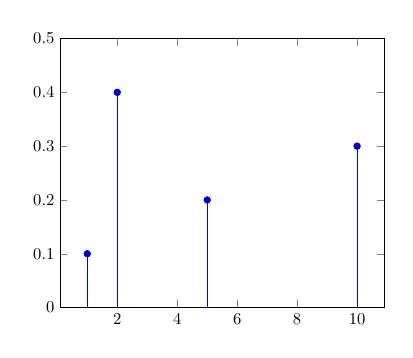
\begin{tikzpicture}[scale = 0.6]
\begin{axis}[ymin = 0, ymax = 0.5,
		y tick label style={
        /pgf/number format/.cd,
            fixed,
            precision=2,
        /tikz/.cd
    }]
\addplot+[ycomb] plot coordinates {(1,1/10) (2,4/10) (5,2/10) (10,3/10)}; 
\end{axis}
\end{tikzpicture}
\end{minipage}
\end{center}
\end{examp}

\subsection*{Cumulative Distribution Functions}\label{DiscreteExpectationSec}

\begin{defn}\index{Cumulative Distribution Function}\index{Distribution Function}
The cumulative distribution function (abbreviated cdf) $F_X$ for the random variable $X$ is defined by $F_X(x) = P(X \leq x)$.
\end{defn}

Notice that we use capital letters for the cdfs and lower case letters for pmfs. This is conventional and we'll always do it. It's also worth mentioning that the word `cumulative' is frequently dropped, and the cdf is called the distribution function.

\begin{examp} Suppose we roll a pair of dice, and let $X$ be the minimum of the two values that appear on the dice. Find the pmf $f_X$ and the cdf $F_X$.
\par
\noindent The random variable $X$ takes integer values between 1 and 6 inclusive, and referring back to the table in Section \ref{sec 1.1}, we can find the probability $X$ takes the value $x$ by counting the number of cells where the smaller of the two values rolled is equal to $x$. We have $P(X = 1) = \frac{11}{36}$, $P(X = 2) = \frac{9}{36}$, $P(X = 3) = \frac{7}{36}$, and so on.
\par
\noindent The graph of the pmf $f_X$ is shown on the left, and the cdf $F_X$ is shown on the right.

\begin{center}
\begin{tikzpicture}[scale = 0.7]
\begin{axis} [ymin = 0.01, ymax = 0.35, xmin=0, xmax = 7,
		y tick label style={
        /pgf/number format/.cd,
            fixed,
            precision=2,
        /tikz/.cd
    }]
\addplot+[ycomb] plot coordinates {(1,11/36) (2,9/36) (3,7/36) (4,5/36) (5,3/36) (6,1/36)}; 
\end{axis} 
\end{tikzpicture}\ \ \ \ \ \  \begin{tikzpicture}[scale = 0.7]
\begin{axis}[
    clip=false,
    jump mark left,
    ymin=0,ymax=1,
    xmin=0, xmax=7,
    every axis plot/.style={very thick},
    cdf,
    table/create on use/cumulative distribution/.style={
        create col/expr={\pgfmathaccuma + \thisrow{f(x)}}   
    }
]
\addplot [cdf init, blue] table [y=cumulative distribution]{
x f(x)
0 0
1 11/36
2 9/36
3 7/36
4 5/36
5 3/36
6 1/36
7 0
};
\end{axis}
\end{tikzpicture}
\end{center}
\par
\noindent Notice that $F_X(2.5) = P(X \leq 2.5) = P(X = 1) + P(X = 2) = \frac{11}{36} + \frac{9}{36} \simeq 0.56$. The cumulative distribution function adds up the probabilities that $X$ takes any value smaller than or equal to its input. 
\end{examp}
\par
Consider two real numbers $a$ and $b$ with $a \leq b$. Given any random variable $X$,  $F_X(a) \leq F_X(b)$, because if $X$ is smaller than $a$ then it must also be smaller than $b$, in other words, the event $X \leq a$ is a subset of the event $X \leq b$, and hence it cannot be more likely. This means that a cdf is always non-decreasing. This and other key properties that all cdfs share are listed in the proposition below.

\begin{prop}\label{cdfproperties}
For any random variable $X$, the distribution function $F_X$ satisfies the following properties.
\vspace{-0.5em}
\begin{enumerate}[(i)]
\item $F_X(x) \geq 0$ for all $x \in \mathbb{R}$.
\item $F_X$ is non-decreasing.
\item $\displaystyle\lim_{x \to -\infty} F_X(x) = 0$ and $\displaystyle\lim_{x \to \infty} F_X(x) = 1$.
\item $F_X(x)$ is right-continuous, meaning $\displaystyle\lim_{x \to a^{+}} F_X(x) = F_X(a)$.
\end{enumerate}
\end{prop}

\par
In fact, these properties completely characterize distribution functions, that is, any function satisfying all four properties is the cdf of some random variable. You should be able to justify the first three properties from the definition of a cdf, but it's not immediately clear clear why we might expect the fourth property to hold.

\begin{thm}
If $X$ is any random variable, then its distribution function $F_X$ is right-continuous.
\end{thm}
\begin{pf}
Take any $a \in \mathbb{R}$, and consider a decreasing sequence of real numbers $\{x_i\}_{i=1}^{\infty}$ that converges to $a$. If you'd like a concrete example to think about, consider the sequence $a+1$, $a+\frac{1}{2}$, $a+\frac{1}{4}$, $a+\frac{1}{8}$, and so on.
\par
\noindent Define events $\{A_i\}_{i=1}^{\infty}$ from this sequence by letting $A_i$ be the event `$X$ is less than $x_i$'. Since the sequence $\{x_i\}_{i=1}^{\infty}$ is decreasing, $\{A_i\}_{i=1}^{\infty}$ is a decreasing sequence of events, so by Theorem \ref{continuity},
\eqnspar{P(\cap_{i=1}^{\infty}A_i) = \lim_{i \to \infty}P(A_i).}
\par
\noindent But the event $\cap_{i=1}^{\infty}A_i$ occurs when all $A_i$ occur, which means that $X$ is smaller than any element of the sequence $\{x_i\}_{i=1}^{\infty}$, and this means $X \leq a$. Therefore we have
\eqnspar{P(X \leq a) = \lim_{i \to \infty}P(A_i).}
\par
\noindent Now $P(X \leq a) = F_X(a)$ by definition of the cdf of X, and since $A_i$ occurs when $X \leq x_i$, we have $P(A_i) = P(X \leq x_i) = F_X(x_i)$ as well. Thus,
\eqnspar{F_X(a) = \lim_{i \to \infty}F_X(x_i).}
\par
\noindent Since $\{x_i\}_{i=1}^{\infty}$ was an arbitrary decreasing sequence that converges to $a$, the limits $\lim_{i \to \infty}F_X(x_i)$ and $\lim_{x \to a^+}F_X(x)$ are equal (in both cases we are approaching $a$ from the right) so we have the desired equality.
\eqnspar{F_X(a) = \lim_{x \to a^{+}}F_X(a).}
\end{pf}

\par
When dealing with cdfs, $F_X(a+)$ is used as an abbreviation of $\lim_{x \to a^{+}}F_X(x)$, and similarly, $F_X(a-)$ is used to abbreviate $\lim_{x \to a^{-}}F_X(x)$. Using this notation we can express the probabilities many events succinctly in terms of the cdf.

\begin{center}
\begin{tabular}{c|c}
Event & Probability \\
\hline
$X \leq a$ & $F_X(a)$ \\
$X < a$ & $F_X(a-)$ \\
$X = a$ & $F_X(a) - F_X(a-)$ \\
$X \geq a$ & $1 - F_X(a-)$ \\
$X > a$ & $1 - F_X(a)$ \\
$a < X < b$ & $F_X(b-) - F_X(a)$ \\
$a \leq X \leq b$  & $F_X(b) - F_X(a-)$ \\
\end{tabular}
\end{center}

Of particular interest is that fact that $P(X=a) = F_X(a) - F_X(a-)$. This is a formal statement of the observation that the possible values of a discrete random variable $X$ are the values where $F_X$ has a discontinuity, and the distance the graph jumps at $a$ is $P(X = a)$.

\begin{examp}
Consider the function whose graph is given below. Check that this function a cdf for some random variable. If we call the random variable with this cdf $Z$, find $P(1 < Z < 2)$, $P(Z = 4)$, and $P(Z > 1)$.

\begin{center}
\begin{tikzpicture}[scale = 0.7]
\begin{axis}[
    clip=false,
    jump mark left,
    ymin=0,ymax=1,
    xmin=-3, xmax=6,
    every axis plot/.style={very thick},
    cdf,
    table/create on use/cumulative distribution/.style={
        create col/expr={\pgfmathaccuma + \thisrow{f(x)}}   
    }
]
\addplot [cdf init,blue] table [y=cumulative distribution]{
x f(x)
-3 0
-2 1/6
0 1/6
2 1/3
4 1/6
5 1/6
6 0
};
\end{axis}
\end{tikzpicture}
\end{center}

\par
\noindent It's easy to see that this function is non-negative, non-decreasing, and tends to $0$ as x $\to -\infty$ and 1 as $x \to \infty$ (we're assuming the graph continues off to the left and right along the horizontal lines shown). Furthermore, it's right-continuous since at each jump the value of the function is equal to the limit from the right.
\vspace{0.5em}
\eqns{P(1 < Z < 2) &= F_Z(2-) - F_Z(1) & \qquad P(Z = 4) &= F_Z(4) - F_Z(4-) \\
&=\frac{2}{6} - \frac{2}{6} = 0 &  &=\frac{5}{6} - \frac{4}{6} = \frac{1}{6}}
\vspace{1.5em}
\eqns{P(Z > -1) &= 1 - F_Z(-1) \\ & = 1 - \frac{1}{6} = \frac{5}{6} }
\end{examp}

\section{Expected Value}\label{ExpectedValueSec}
\par
Suppose we flip a fair coin three times and count the number of heads that appear. If we repeat this experiment many times, what do we expect the average number of heads to be?
\par
If we let $X$ be the number of heads observed when a single trial of this experiment is performed, then $X$ is a discrete random variable whose distribution is given in the table below.
\vspace{-0.5em}
\renewcommand*{\arraystretch}{1.35}
\begin{center}
\begin{tabular}{c|c}
$x$ & $P(X = x)$ \\
\hline
$0$ & $\frac{1}{8}$ \\
$1$ & $\frac{3}{8}$ \\
$2$ & $\frac{3}{8}$ \\
$3$ & $\frac{1}{8}$
\end{tabular}
\end{center}
\renewcommand*{\arraystretch}{1}
\par
If we perform the experiment many times, then we should expect to observe no heads about $12.5\%$ of the time, one head $37.5\%$ of the time, and so on (this is the frequentist interpretation of probability). If we weight each possible number of heads by the probability it occurs, we obtain
\eqnspar{0 \cdot \frac{1}{8} + 1 \cdot \frac{3}{8} + 2 \cdot \frac{3}{8} + 3 \cdot \frac{1}{8} = \frac{12}{8} = 1.5.}
\par
So not surprisingly we should, on average, obtain 1.5 heads in every three flips of a fair coin. This notion of the average value of a random variable is formalized in the definition below.

\begin{defn}\label{expectedvaluedef}
Given a discrete random variable $X$ which takes values in the set $A = \{x_1, x_2, x_3, ...\}$, the expected value of $X$, also called the mean of X, is denoted $E(X)$ or $\mu_X$, and is given by multiplying each possible value of X by its probability.
\eqnsgap{\boxed{E(X) = \sum_{x \in A}^{\ } x \cdot P(X = x) = \sum_{x \in A} x \cdot f_X(x)}}
\end{defn}

\rmk The sum in the definition above could be infinite, in which case it may or not converge. If the sum is not absolutely convergent, then $E(X)$ is undefined.

\begin{examp}
Alice needs to decide whether to buy individual metro tickets at \$3.25 each, or an unlimited weekend pass at \$13.75. If she knows she'll take the metro either three, four, or five times this weekend with equal probability, what is the best decision?
\par
\noindent Let $X$ represent the amount of money Alice will spend if she buys individual tickets. Then $X$ is equally likely to take the three values $9.75$, $13$, and $16.25$. Therefore,
\eqnspar{E(X) = 9.75 \cdot \frac{1}{3} + 13 \cdot \frac{1}{3} + 16.25 \cdot \frac{1}{3} = 13.}
\par
\noindent On the other hand, if she purchases the unlimited pass, she'll pay $\$13.75$. Thus, if Alice is interested in saving money, she should opt for the individual tickets.
\end{examp}

\begin{examp}
Consider the random variable $Z$ whose cdf is given. Find $E(Z)$.
\renewcommand*{\arraystretch}{1.35}
\eqns{F_Z(z) = \left\{
\begin{array}{cl}
      0 & \text{ if \ } z < -3 \\
			\frac{1}{3} & \text{ if \ } -3 \leq z < 1 \\
			\frac{1}{2} & \text{ if \ } 1 \leq z < 5 \\
			\frac{5}{6} & \text{ if \ } 5 \leq z < 6 \\
      1 & \text{ if \ } z \geq 6 \\ \end{array} 
\right.}
\renewcommand*{\arraystretch}{1}
\par
\noindent Since $P(Z = a) = F_Z(a) - F_Z(a-)$ we can recover the pmf $f_Z$ by examining the discontinuities of $F_Z$. From the pmf we compute $E(Z)$.
\renewcommand*{\arraystretch}{1.35}
\eqns{f_Z(z) = \left\{
\begin{array}{cl}
			\frac{1}{3} & \text{ if \ } z = -3 \\
			\frac{1}{6} & \text{ if \ } z = 1 \\
			\frac{1}{3} & \text{ if \ } z = 5 \\
      \frac{1}{6} & \text{ if \ } z = 6 \\ \end{array} 
\right.}
\vspace{1em}
\eqns{E(Z) = \sum_{z \in A} z \cdot f_Z(z) = -3 \cdot \frac{1}{3} + 1 \cdot \frac{1}{6} + 5 \cdot \frac{1}{3} + 6 \cdot \frac{1}{6} = \frac{11}{6}}
\renewcommand*{\arraystretch}{1}
\end{examp}

\par
\noindent One immediate application of expected value is to games of chance. Given such a game, if we let $X$ represent the player's profit from playing the game once, then if $E(X) > 0$ it's a winning bet, if $E(X) < 0$ it's a losing bet, and if $E(X) = 0$, it's a fair game. 

\begin{examp}
On a roulette wheel, there are 18 black numbers, 18 red numbers, and 2 green numbers. Any wager made on black will double if successful. Find the expected value of a \$20 bet on black, assuming each of the numbers on the roulette wheel is equally likely to be selected.
\par
\noindent Let $X$ represent the profit from a bet of $\$20$ on black. Then $X$ can take only values in $A = \{20, -20\}$ since the bet is either won or lost. There are a total of 38 possible outcomes, 18 of which result in a win, so $P(X = 20) = \frac{18}{38}$ and $P(X = -20) = \frac{20}{38}$.
\eqns{E(X) = 20 \cdot \frac{18}{38} + (-20) \cdot \frac{20}{38} = -\frac{40}{38} \simeq -1.05}
\par
\noindent Therefore, this is a losing bet. If you were to sit at a roulette table and repeatedly make \$20 bets on black for a very long time, you should expect your losses to total about \$1 per game played. Conversely for the casino, they should expect to make a \$1 profit for every \$20 bet on black played.
\end{examp}

\begin{examp}
(St-Petersburg lottery) A coin is flipped until the first tail appears. You are initially given \$1 before the coin is flipped for the first time, and every time a head appears, the prize doubles. When the first tail appears, you receive the prize. If the sequence of flips that appears is $HHHT$, for example, you would receive \$8. What is the expected value of the prize?
\par
\noindent If we define a random variable $X$ on the sample space $\Omega = \{T, HT, HHT, ...\}$ whose value is the prize, then $X$ can take any value in $A = \{1,2,4,8,16, \,...\}$, i.e., any value of the form $2^k$ for $k \in \mathbb{N}$. Furthermore, $X = 2^k$ when the outcome is a sequence with $k$ heads followed by a tail. Thus, $P(X = 2^k) = \left(\frac{1}{2}\right)^{k+1}$.
\eqns{E(X) &= \sum_{x \in A} x P(X = x) \\
&= \sum_{k = 0}^{\infty} 2^k P(X = 2^k) \\
&= 1 \cdot \frac{1}{2} + 2 \cdot \frac{1}{4} + 4 \cdot \frac{1}{8} + 8 \cdot \frac{1}{16}  + ... \\
&= \frac{1}{2} + \frac{1}{2} + \frac{1}{2} + \frac{1}{2} + ... \rightarrow \infty}
\par
\noindent The expected value is undefined, since the sum diverges by growing arbitrarily large. 
\end{examp}
\par
This is a very strange result, since it implies that even if you're required to pay \$1\,000\,000 to play this game, it's still a winning bet. How can this be?
\par
Notice that this is not a game one could actually play, as there's only a finite amount of money in the world. If this example is redone with an upper limit on the payout, the expected value will exist and give the average payout in the game. Using the current global GDP as the payout limit, the result is around \$45.
\par
It's also worth considering that someone with \$\,$2 \times 10^{100}$ has twice as much money as someone with \$\,$1 \times 10^{100}$ in a literal sense, but both could spend the rest of their lives throwing briefcases of money into a fire and neither would make a dent in their net worth. In practice, twice as much money doesn't have twice as much value. Regardless, if one were actually able to play this game as stated, and play it as many times as one desires, it would be rational do so even if every play cost \$1\,000\,000, since one would \emph{eventually} win an amount so large that the sum of all prior losses would be rendered insignificant. 

\subsection*{Properties of the Expected Value}

\begin{thm}\label{LawUnconsciousStatistician}\index{Law of the Unconscious Statistician}
(Law of the Unconscious Statistician) If $X$ is a discrete random variable that takes values in the set $A = \{x_1, x_2, x_3, ...\}$ and $g: \mathbb{R} \to \mathbb{R}$, the random variable $Y = g(X)$ has 
\eqns{\boxed{E(Y) = \sum_{x \in A}^{\ } g(x)f_X(x).}}
\end{thm}
\par
Notice that the pmf in the sum is the pmf for $X$. We're finding the expected value of $Y$ so we would imagine the pmf of $Y$ would be involved here, but it isn't, and hence the name of the theorem. Using this result, we can calculate the expected value of $Y$ without knowing its pmf, which saves a lot of work.
\par
\vspace{0.5em}
\begin{pf}
Consider $g(A) = \{g(x_1), g(x_2), g(x_3), ...\}$, the set of possible values for $Y$. From the definition of expected value, we have
\eqnspar{E(Y) = \sum_{y \in g(A)} y \cdot f_Y(y).}
\par
\noindent Let $g^{-1}(y) = \{x \, | \, g(x) = y\}$, the set of all $x \in A$ that are sent to $y$ by the function $g$. By definition, $f_Y(y)$ is equal to $P(Y=y)$, which is the sum of the probabilities of all values of $X$ which $g$ sends to $y$ (we saw this in Example \ref{FunctionRVEx}). Formally, 
\eqnspar{f_Y(y) = P(Y = y) = P(g(X) = y) = P(X \in g^{-1}(y)) = \sum_{x \in g^{-1}(y)} P(X = x).}
\par
\noindent Therefore, we have
\eqns{E(Y) &= \sum_{y \in g(A)} y \cdot f_Y(y) = \sum_{y \in g(A)} y \cdot \sum_{x \in g^{-1}(y)} P(X = x) \\
&= \sum_{y \in g(A)} \sum_{x \in g^{-1}(y)} y \cdot P(X = x) = \sum_{y \in g(A)} \sum_{x \in g^{-1}(y)} g(x) \cdot P(X = x).}
\par
\noindent In the last expression, the first sum is over all $y \in g(A)$, and for each such $y$, the second sum is over all $x \in A$ which are sent to that $y$. But every $x \in A$ is sent to some $y \in g(A)$, so the double sum is just summing over all $x \in A$. Thus,
\eqns{E(Y) = \sum_{y \in g(A)} \sum_{x \in g^{-1}(y)} g(x) \cdot P(X = x) = \sum_{x \in A} g(x) \cdot P(X = x) = \sum_{x \in A} g(x) \cdot f_X(x).}
\end{pf}

\begin{examp}
Suppose that $X$ is a random variable that takes the values $-2$, $-1$, $0$, $1$, and $2$ with equal likelihood. Find the expected value of $Y = \frac{1}{1+X^2}$.
\par
\noindent Note that the pmf $f_X$ has $f_X(x) = \frac{1}{5}$ for $x \in \{-2,-1,0,1,2\}$, and that $Y = g(X)$, where $g(X) = \frac{1}{1+X^2}$. Using the Law of the Unconscious Statistician,
\eqnsgap{E(Y) &= \sum_{x \in A} g(x)f_X(x) \\
&= \frac{1}{1+(-2)^2} \cdot \frac{1}{5} + \frac{1}{1+(-1)^2} \cdot \frac{1}{5} + \frac{1}{1+(0)^2} \cdot \frac{1}{5} + \frac{1}{1+(1)^2} \cdot \frac{1}{5} + \frac{1}{1+(2)^2} \cdot \frac{1}{5} \\
&=\frac{1}{25} + \frac{1}{10} + \frac{1}{5} + \frac{1}{10} + \frac{1}{25} = \frac{12}{25}}
\end{examp}
\vspace{0.25em}
\par
\begin{cor}\label{LinearityI}
(Linearity of Expectation, Pt.\,I) If $X$ is a discrete random variable, and $Y = aX + b$ for some $a,b \in \mathbb{R}$, then $E(Y) = aE(X)+b$.
\end{cor}
\begin{pf} Applying the Law of the Unconscious Statistician, expanding, and then splitting up the sum, we have
\eqns{E(Y) &= \sum_{x \in A}g(x)f_X(x) = \sum_{x \in A}(ax+b) \cdot f_X(x) = \sum_{x \in A} ax\cdot f_X(x) + b f_X(x) \\
&= \sum_{x \in A} ax\cdot f_X(x) + b \sum_{x \in A}f_X(x) = a\sum_{x \in A} x\cdot f_X(x) + b \sum_{x \in A}f_X(x) \\
&=aE(X) + b(1) = aE(X)+b.}
\par
\noindent Note that $\sum_{x \in A}f_X(x) = 1$ since $f_X$ is a probability mass function.
\end{pf}

With a clever application of this result, we can resolve the problem posed at the beginning of this chapter, which is a variation of the St-Petersburg lottery.

\begin{examp}
In a certain game, a coin is flipped until the first tail appears. If $n$ heads occurred before this first tail which ends the game, the payout is $\$n$. What is the expected value of the payout?
\par
\noindent Let $X$ be a random variable defined over the sample space $\Omega = \{T, HT, HHT, ...\}$ which gives the value of the payout. Then we have $P(X = 0) = \frac{1}{2}$, $P(X = 1) = \frac{1}{4}$, $P(X = 2) = \frac{1}{8}$, and in general $P(X = k) = \frac{1}{2^k}$. Thus, $f_X(k) = \frac{1}{2^{k+1}}$ for $k \in \mathbb{N}$, and hence
\eqns{E(X) = \sum_{x \in A}x f_X(x) = \sum_{k = 1}^{\infty}k \cdot \frac{1}{2^{k+1}} = \frac{1}{4} + \frac{2}{8} + \frac{3}{16} + \frac{4}{32} + \frac{5}{64} + ...}
\par
\noindent In the St-Petersburg lottery, the infinite sum was clearly divergent, but this time it's not so easy to evaluate, in fact it's quite difficult.
\par
\noindent Let's try another approach. Suppose the game has just begun and the first flip occurs. If the result is tails, then the game is over and you gain nothing, but if the result is heads, your payout goes up by $\$1$. In this second case, it's as if you've put $\$1$ into your pocket and started the game again, since each subsequent head also pays the same amount, $\$1$. If your payout in a new game is given by $X$, then your payout in a game in which a single head has already been flipped is given by $X+1$.
\par
\noindent On the first flip then, there's a $\frac{1}{2}$ chance that a tail is flipped, and the payout is zero, and there's a $\frac{1}{2}$ chance that a head is flipped, and the payout is $X+1$. Therefore,
\eqns{E(X) &= \textstyle\frac{1}{2} \cdot 0 + \frac{1}{2}\cdot E(X+1)\\
E(X) &= 0 + \textstyle\frac{1}{2}\cdot (E(X)+1) \\
E(X) &= \textstyle\frac{1}{2}E(X) + \textstyle\frac{1}{2}\\
E(X) - \textstyle\frac{1}{2}E(X)&= \textstyle\frac{1}{2} \\
E(X) &= 1}
\par
\noindent Corollary \ref{LinearityI} was used to pass from the first to the second line, and from there on we simply isolated $E(X)$.
\end{examp}
\par
Notice that we can also obtain the expected value of any discrete random variable by summing over all possible outcomes $\omega \in \Omega$, instead of all possible values of $X$. This approach is sometimes more natural and sometimes more difficult.
\par
Consider for example a random variable $X$ that counts the number of heads in two flips of a fair coin. Using Definition \ref{expectedvaluedef}, and letting $A = \{0,1,2\}$ denote the possible values of $X$, we have
\eqnspar{E(X) = \sum_{x \in A} x f_X(x) = 0 \cdot \frac{1}{4} + 1 \cdot \frac{1}{2} + 2 \cdot \frac{1}{4} = 1.}
\par
On the other hand, we could let $X(\omega)$ denote the value of $X$ when the outcome $\omega$ occurs, and sum over all outcomes in the sample space $\Omega = \{HH, HT, TH, TT\}$.
\eqns{E(X) = \sum_{\omega \in \Omega} X(\omega) P(\omega) &= X(HH) \cdot \frac{1}{4} + X(HT) \cdot \frac{1}{4} + X(TH) \cdot \frac{1}{4} + X(TT) \cdot \frac{1}{4} \\
& = 2 \cdot \frac{1}{4} +1 \cdot \frac{1}{4} +1 \cdot \frac{1}{4} +0 \cdot \frac{1}{4} = 1.}
\par
\begin{prop} For a discrete random variable $X$ defined on the sample space $\Omega$, 
\eqnsgap{E(X) = \sum_{\omega \in \Omega} X(\omega)P(\omega)}
\end{prop}
\begin{thm}\label{LinearityII}
(Linearity of Expectation, Pt.\,II) If $X$  and $Y$ are discrete random variables defined over the same sample space $\Omega$, then $E(X+Y) = E(X) + E(Y)$.
\end{thm}
\begin{pf} Using the formula above to compute the expected value of $X+Y$, we have
\eqns{E(X+Y) &= \sum_{\omega \in \Omega} (X(\omega)+Y(\omega)) P(\omega) \\ &=  \sum_{\omega \in \Omega} X(\omega)P(\omega)+Y(\omega) P(\omega) \\ &= \sum_{\omega \in \Omega} X(\omega)P(\omega)+ \sum_{\omega \in \Omega} Y(\omega) P(\omega) \\
&= E(X)+E(Y).}
\end{pf}

This result also extends to sums of any number of random variables defined on the same sample space. In general, the expected value of a sum of random variables is the sum of their expectations.

\begin{examp}
If we roll six dice and sum the results, what is the expected value of the sum? 
\par
\noindent Let $X_i$ denote the result of the $i^{th}$ roll, and let $Y = X_1 + X_2 + X_3 + X_4+ X_5 + X_6$. Every $X_i$ has the same expected value, which we calculate below.
\vspace{0.5em}
\eqns{E(X_i) = 1 \cdot \frac{1}{6} + 2 \cdot \frac{1}{6}+ 3 \cdot \frac{1}{6}+ 4 \cdot \frac{1}{6}+ 5 \cdot \frac{1}{6}+ 6 \cdot \frac{1}{6} = \frac{21}{6} = 3.5}
\par
\noindent Thus, $E(Y) = 3.5 + 3.5 + 3.5 + 3.5 + 3.5 + 3.5 = 21$.
\end{examp}


\begin{examp}
Suppose that Bob draws four marbles, with replacement, from an urn containing one blue, one green, one yellow, and one red marble. What is the expected number of different colours that will appear among Bob's selections?
\par
\noindent We'll solve this problem using a clever idea known as the method of indicators. Let $I_b$ be an indicator variable for the event `at least one blue marble is drawn', so $I_b$ takes the value $1$ if a blue marble is drawn and $0$ if not. Define $I_g$, $I_y$, and $I_r$ similarly, so we have an indicator variable for each colour.
\par
\noindent The expected value of $I_b$ is easy to calculate, since $I_b = 0$ when no blue marbles are drawn, so $P(I_b = 0) = (\frac{3}{4})^4 = \frac{81}{256}$, and hence $P(I_b = 1) = 1 - \frac{81}{256} = \frac{175}{256}$. Therefore, $E(I_b) = 0 \cdot \frac{81}{256} + 1 \cdot \frac{175}{256} =\frac{175}{256}$. The same is true for $I_g$, $I_y$, and $I_r$.
\par
\noindent If we define $X$ as the number of different colours that appear among the four draws, then $X = I_b + I_g + I_y + I_r$, hence by linearity of expectation,
\eqnsgap{E(X) &= E(I_b + I_g + I_y + I_r) \\ 
&= E(I_b) + E(I_g) + E(I_y) + E(I_r) \\
&= 4\left(\frac{175}{256}\right) = \frac{700}{256} \simeq 2.73.}
\end{examp}
\par
Notice that in the example above, though $I_b$, $I_y$, $I_g$, and $I_r$ are indicators for events that are not independent, linearity of expectation allows us to compute the expected value of their sum without thinking about how the value of one affects any of the others.
\par
Now consider a discrete random variable $X$ whose range is $\{1,2,\,...\,,n\}$ for some positive integer $n$, and notice that if we define an indicator $I_k$ for the event $X \geq k$ for each $k$ from $1$ to $n$, then $X = I_1 + I_2 + ... + I_n.$
\par
To illustrate, say for example that $X$ takes the value $2$. Then $I_1$ and $I_2$ both take the value one, and all $I_k$ for $k > 2$ are zero, so $X = I_1 + I_2 + I_3 + ... + I_n = 1 + 1 + 0 + ... + 0 = 2$. Using linearity of expectation, we have $$E(X) = E(I_1 + I_2 + ... + I_n) = E(I_1) + E(I_2) + ... + E(I_n).$$
What is $E(I_k)$ for each $k \in \{1,2,\,...\,,n\}$? By definition, $I_k = 1$ if $X \geq k$ and $I_k = 0$ if $X < k$, hence $E(I_k) = 1\cdot P(X \geq k) + 0\cdot P(X<k) = P(X \geq k)$. Thus, $E(X) = E(I_1) + E(I_2) + ... + E(I_n) = P(X\geq 1) +P(X\geq 2) + ... + P(X\geq n)$.

\begin{prop}\label{Discrete Tail Sum Formula}\index{Tail Sum Formula}\index{Expected Value!tail sum formula for}(Tail Sum Formula)
Given a discrete random variable $X$ which takes values in $\{1,2,\,...\,,n\}$,
\eqnsgap{\boxed{E(X) = \sum_{k=1}^{n} P(X\geq k).}}
In fact, the assumption that there is an upper bound, $n$, on the values $X$ can take turns out to be unnecessary, and we can sum over all positive integers.
\end{prop}
\par
Typically we compute expected values directly using Definition \ref{expectedvaluedef}, but there are some cases where the method of indicators or this tail sum formula make calculations substantially faster.
\begin{examp}
For fair dice are rolled. What is the expected value of the smallest of the four resulting numbers?
\par
\noindent Let $X$ be a random variable representing the smallest of the four resulting numbers. Then $X$ takes values in the set $\{1,2,3,4,5,6\}$, but writing the distribution of $X$ involves doing a lot of combinatorics. 
\par
\noindent On the other hand, finding $P(X \geq k)$ for each $k \in \{1,2,3,4,5,6\}$ is quite easy. For example, the event $X \geq 2$ occurs when every die shows a result higher than or equal to 2. Since the die rolls are independent, we have $P(X\geq2) = \frac{5}{6}\cdot\frac{5}{6}\cdot\frac{5}{6}\cdot \frac{5}{6} = (\frac{5}{6})^4$. Using the tail sum formula yields
\eqnsgap{E(X) &= \sum_{k=1}^{6}P(X \geq k) \\
&= P(X \geq 1) + P(X \geq 2) + ... + P(X \geq 6) \\
&= 1 + \left(\frac{5}{6}\right)^4+\left(\frac{4}{6}\right)^4+\left(\frac{3}{6}\right)^4+\left(\frac{2}{6}\right)^4+\left(\frac{1}{6}\right)^4 \\ 
&\approx 1.76}
\end{examp}

\section{Variance}

The expected value of a random variable gives us a way quantifying what's meant by the center of a distribution. 
\par
In fact, if the vertical lines in the graph of the pmf $f_X$ each represent literal masses whose weights are proportional to their heights, then the value of $E(X)$ is the point on the $x$-axis where the distribution balances, and that's certainly a reasonable definition for the center.
\vspace{0.5em}
\begin{center}
\begin{tikzpicture}[scale = 0.7]
\begin{axis} [ymin = 0, ymax = 0.5,
		y tick label style={
        /pgf/number format/.cd,
            fixed,
            precision=2,
        /tikz/.cd
    }]
\addplot+[ycomb] plot coordinates {(2,1/7) (3,2/7) (5,1/7) (6,3/7)}; 
\end{axis} 
\node (a) at (3.85,-0.3) {};
\node (b) at (4.05,0) {};
\node (c) at (4.25,-0.3) {};
\node (d) at (4.05,-1) {};
\draw (a.center)--(b.center)--(c.center);
\draw (b.center)--(d.center);
\end{tikzpicture}
\end{center}
\par
We can also use expected value to quantify the amount of dispersion present in a probability distribution. Consider for example the two random variables $X$ and $Y$ whose pmfs are given on the left and right respectively.

\begin{center}
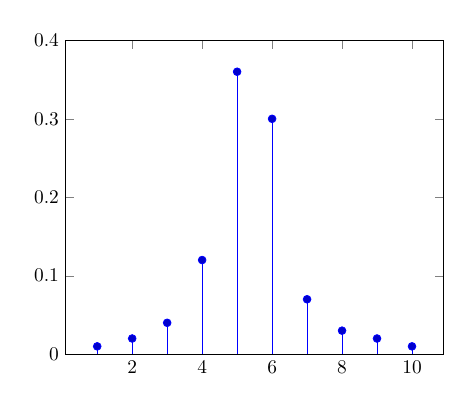
\begin{tikzpicture}[scale = 0.7]
\begin{axis} [ymin = 0, ymax = 0.4,
		y tick label style={
        /pgf/number format/.cd,
            fixed,
            precision=2,
        /tikz/.cd
    }]
\addplot+[ycomb] plot coordinates {(1, 0.01) (2, 0.02) (3, 0.04) (4, 0.12) (5, 0.36) (6, 0.30) (7, 0.07) (8, 0.03) (9, 0.02) (10, 0.01)}; 
\end{axis}
\end{tikzpicture}\ \ \ \ \ \ 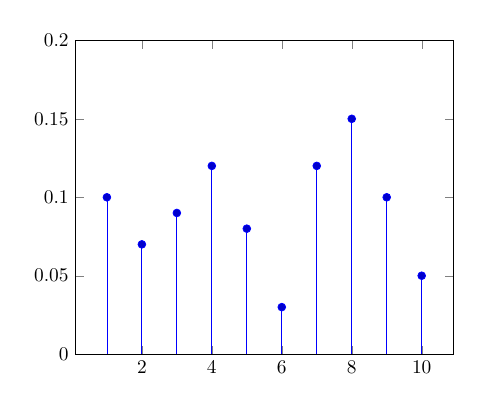
\begin{tikzpicture}[scale = 0.7]
\begin{axis} [ymin = 0, ymax = 0.2,
		y tick label style={
        /pgf/number format/.cd,
            fixed,
            precision=2,
        /tikz/.cd
    }]
\addplot+[ycomb] plot coordinates {(1, 0.10) (2, 0.07) (3, 0.09) (4, 0.12) (5, 0.08) (6, 0.03) (7, 0.12) (8, 0.15) (9, 0.1) (10, 0.05)}; 
\end{axis}
\end{tikzpicture}
\end{center}

The values of $X$ tend to be clustered close to the center of the distribution, only very rarely will straying under 4 or over 7. On the other hand, $Y$ takes on values far from the center of its distribution quite often. In other words, the distance between the value of $X$ and the center of its distribution is usually smaller than the distance between the value of $Y$ and its center of its distribution. 

\rmk In the discussions in this section, many expressions are made clearer by using the notation $\mu_X$ in place of $E(X)$, so keep in mind that $\mu_X$ is the expected value of $X$, which is a constant value at the center of the distribution of $X$.

\par
Thus, we can quantify the dispersion of a random variable $X$ by calculating the average distance from $X$ to $\mu_X$, that is, the expected value of the difference between $X$ and its expected value. In practice, it's more common to work with the expected value of the \emx{squared} difference between $X$ and its average.

\begin{defn}\index{Random Variable!variance of}\index{Random Variable!standard deviation of}\index{Variance}\index{Standard Deviation}\label{VarianceDef} The variance of a discrete random variable $X$ is denoted $\Var(X)$ or $\sigma^{2}_{X}$, and defined by $\Var(X) = E[(X - \mu_X)^2]$. The standard deviation of $X$ is then defined by $\sigma_X = \sqrt{\sigma^{2}_X} = \sqrt{\Var(X)}$.
\end{defn}

\par Why square the differences between $X$ and $\mu_X$? It ensures that any deviations, either left or right of $\mu_X$, are always counted positively. If we opt not to square, and ensure the differences are positive using the absolute value, we could calculate $E[\,|X-\mu_X|\,]$, which is called the mean absolute deviation\index{Random Variable!mean absolute deviation of}\index{Mean Absolute Deviation}.

\par Why variance and standard deviation? Why not use the mean absolute deviation defined above, or some other method to measure dispersion? We'll see later on that in fact, the variance measures exactly how difficult a random variable is to predict, in a mathematically precise sense. The ultimate goal in statistics is often to build predictive models, so for this reason variance is a practical measure. The standard deviation also plays a key role in many of the statistical testing procedures we'll see later in the course.

\begin{examp} Determine the expected value, variance, and standard deviation of the random variable $X$ whose pmf is given below.
\renewcommand*{\arraystretch}{1.35}
\eqns{f_X(x) = \left\{
\begin{array}{cl}
      \frac{2}{8} & \text{ if \ } x = 1 \\
			\frac{1}{8} & \text{ if \ } x = 3 \\
			\frac{3}{8} & \text{ if \ } x = 5 \\
			\frac{2}{8} & \text{ if \ } x = 6 \\
      0 & \text{ otherwise} \\ \end{array} 
\right.}
\renewcommand*{\arraystretch}{1}
\par
\noindent First, $E(X) = 1 \cdot \frac{2}{8} + 3 \cdot \frac{1}{8} + 5 \cdot \frac{3}{8} + 6 \cdot \frac{2}{8} = 4$, that is, $\mu_X = 4$. Then we can calculate the variance below.
\eqnsgap{\Var(X)&=E[(X-\mu_x)^2] \\
&=(1-4)^2 \cdot \frac{2}{8} + (3-4)^2 \cdot \frac{1}{8} + (5-4)^2 \cdot \frac{3}{8} + (6-4)^2 \cdot \frac{2}{8} \\
&=9 \cdot \frac{2}{8} + 1 \cdot \frac{1}{8} + 1 \cdot \frac{3}{8} + 4 \cdot \frac{2}{8} = \frac{31}{8}}
\par
\noindent Thus, the standard deviation of $X$ is $\sigma_X = \sqrt{\frac{31}{8}} \simeq 1.968$.
\end{examp}

\begin{examp} In Big Win Bob's game, each player pays $\$1$ to place a bet on a number between 1 and 100, a winning number is selected at random, and the prize for a correct bet is $\$75$. In Conservative Charles' game, each player pays $\$1$ to bet on a number between 1 and 4, a winning number is selected at random, and the prize for a correct bet is $\$3$. Which game would you rather play?
\par
\noindent Let $X$ represent a player's net gain in a single play of Bob's game, and let $Y$ represent a player's net gain in a single play of Charles' game.
\eqns{E(X) &= 74 \cdot \frac{1}{100} + (-1) \cdot \frac{99}{100} = -0.25 \\
E(Y) &= 2 \cdot \frac{1}{4} + (-1) \cdot \frac{3}{4} = -0.25}
\par
\noindent Thus, it does not matter which game you play in the long run. Over a very large number of plays the games are equivalent, either way the player loses 25\textcent\ per game on average. However, the variances of $X$ and $Y$ are not equal.
\eqns{\Var(X) &= (74 - (-0.25))^2 \cdot \frac{1}{100} + (-1-(-0.25))^2 \cdot \frac{99}{100} \simeq 55.69 \\
\Var(Y) &= (2 - (-0.25))^2 \cdot \frac{1}{4} + (-1-(-0.25))^2 \cdot \frac{3}{4} \simeq 1.68}
\par
\noindent This large difference in the variances indicates Big Win Bob's game is much riskier. In Bob's game players win rarely but win big, while in Charles' game players win small amounts quite often.

\end{examp}

\par Calculating the variance by hand is a tedious process, and in practice, one would essentially always use a computer. In simple examples like those above, the following formula can make the calculation significantly faster.

\begin{thm}$\boxed{\Var(X) = E[X^2] - (E[X])^2}$
\end{thm}

\begin{pf} Starting from the definition of $\Var(X)$, expanding $(X-\mu_X)^2$ and using linearity of expectation, we have
\eqns{\Var(X) &= E[(X -\mu_X)^2] \\ &=E[X^2 - 2 \mu_X \cdot X + {\mu_X}^2] \\ &= E[X^2] - E[2 \mu_X \cdot X] + E[{\mu_X}^2].}
\par
\noindent Since $\mu_X$ is a constant, $E[{\mu_X}^2] = {\mu_X}^2$, and using linearity of expectation in the second term, $E[2 \mu_X \cdot X] = 2 \mu_X E[X]$. But $E[X]$ and $\mu_X$ are two different names for the same quantity, so $2 \mu_X E[X] = 2 \mu_X \cdot \mu_X = 2 {\mu_X}^2$. Therefore,
\eqns{\Var(X) &= E[X^2] - E[2 \mu_X \cdot X] + E[{\mu_X}^2] \\
&= E[X^2] - 2 {\mu_X}^2 + {\mu_X}^2 \\
&= E[X^2] - {\mu_X}^2 \\
&= E[X^2] - (E[X])^2}.
\end{pf}

\begin{examp}\label{stdevoneroll}
If $X$ represents the outcome of a roll of a fair die, find $\sigma_X$.
\eqns{E[X] = \sum_{x=1}^{6} x f_X(x) = 1 \cdot \frac{1}{6} + 2 \cdot \frac{1}{6} + 3 \cdot \frac{1}{6} + 4 \cdot \frac{1}{6} + 5 \cdot \frac{1}{6} + 6 \cdot \frac{1}{6} = \frac{7}{2}}
\vspace{0.25em}
\eqnsgap{E[X^2] = \sum_{x=1}^{6} x^2 f_X(x) = 1 \cdot \frac{1}{6} + 4 \cdot \frac{1}{6} + 9 \cdot \frac{1}{6} + 16 \cdot \frac{1}{6} + 25 \cdot \frac{1}{6} + 36 \cdot \frac{1}{6} = \frac{91}{6}}
\par
\noindent Hence, $\Var(X) = E[X^2] - (E[X])^2 = \frac{91}{6} - (\frac{7}{2})^2 = \frac{91}{6} - \frac{49}{4} = \frac{35}{12}$, and square rooting, we obtain the standard deviation $\sigma_X \simeq 1.707$.
\end{examp}

\subsection*{Properties of Variance} 

\begin{prop}Let $X$ be any discrete random variable with $\Var(X) = 0$, then $X$ takes a single value with probability one.
\end{prop}

\begin{pf} Let $A$ be the set of possible values of $X$, and suppose that $k_1, k_2 \in A$ such that $f_X(k_1) \neq 0$ and $f_X (k_2) \neq 0$, i.e. $X$ can take either value with nonzero probability.
\eqnspar{\Var(X) = E[(X - \mu_X)^2] = \sum_{x \in A} (x - \mu_X)^2f_X(x)}
\par
\noindent Every term in the sum on the right is non-negative since squares are non-negative, and $f_X(x) \geq 0$ by definition of a pmf. Furthermore, at least one term is nonzero since $k_1$ and $k_2$ are distinct, so either $k_1  - \mu_X \neq 0$ or $k_2 - \mu_x \neq 0$. Thus, the sum must be positive, so we conclude that if $X$ takes more than one distinct value with nonzero probability, $\Var(X) \neq 0$.
\end{pf}

\begin{thm}\label{VarianceLinearity} For any constants $a, b \in \mathbb{R}$, $\boxed{\Var(aX+b) = a^2\Var(X)}$.
\end{thm}
\begin{pf} This result follows from the definition of variance, using linearity of expectation.
\eqns{\Var(aX+b) &= E[((aX+b) - \mu_{aX+b})^2] \\
&= E[((aX+b) - E(aX+b))^2] \\
&= E[((aX+b) - (aE(X)+b))^2] \\
&= E[((aX - aE(X))^2] \\
&= E[a^2(X - E(X))^2] \\
&= a^2E[(X-E(X))^2] \\
&= a^2E[(X - \mu_X)^2] \\
&= a^2\Var(X)}
\end{pf}

\begin{examp} If $X$ is a random variable with $E(X) = 2$ and $E[X(X-4)]=7$, what is the standard deviation of $Y = 2X+2$?
\par
\noindent Using linearity of expectation,
\eqnspar{E[X(X-4)] = E[X^2 - 4X] = E[X^2] - 4E[X] = E[X^2] - 8.}
\par
\noindent Thus, $E[X^2] - 8 = 7$, so $E[X^2] = 15$, and hence 
\eqnspar{\Var(X) = E[X^2] - (E[X])^2 = 15-4 = 11.}
\par
\noindent Applying the result above, $\Var(Y) = \Var(2X+2) = 4\Var(X) = 44$, so $\sigma_Y = \sqrt{44}$.
\end{examp}

\subsection*{Independent Random Variables}

We've seen in Section \ref{IndependenceOfEvents} that two events $A \subseteq \Omega$ and $B \subseteq \Omega$ are independent if $P(A \given B) = P(A)$, or equivalently, if $P(A \cap B) = P(A)P(B)$. This definition can be extended to random variables.

\begin{defn}\label{IndependenceOfRVs}\index{Independence!of discrete random variables}
Two random variables $X$ and $Y$ defined on the same sample space $\Omega$ are independent if $P(X = x \,\cap\, Y = y) = P(X = x)P(Y = y)$ for all $x$ and $y$.\end{defn}

\begin{examp}Suppose a fair die is rolled twice. Let $X$ be the result of the first roll and $Y$ be the result of the second. Then $X$ and $Y$ are independent random variables, since for any $x$ and $y$ in $\{1,2,3,4,5,6\}$, we have $P(X = x \,\cap\, Y = y) = \frac{1}{36}$, while $P(X = x) = \frac{1}{6}$ and $P(Y=y) = \frac{1}{6}$.
\end{examp}

\begin{examp}Let X be a number chosen at random from the set $\{1,2,3,4,5,6\}$, and let $Y$ be the remainder when $X$ is divided by 3. Then $X$ and $Y$ are not independent random variables, since, for instance, $P(X = 3 \,\cap\, Y = 1) = 0$, because if $X = 3$ then we must have $Y = 0$, while $P(X = 3)P(Y = 1) = \frac{1}{6}\cdot\frac{2}{6}$.
\end{examp}

In the last section we saw that $E(X+Y) = E(X) + E(Y)$ for any random variables $X$ and $Y$. The relationship between $\Var(X)$, $\Var(Y)$, and $\Var(X+Y)$ is generally more complicated. The details require defining the joint distribution of two random variables and an extensive discussion. If you're interested see \cite{Bertsekas} or \cite{Ghahramani}. In the case where $X$ and $Y$ are independent though, $\Var(X+Y) = \Var(X) + \Var(Y)$. To prove this, we need to establish the lemma below.

\begin{lem}\label{ExpectationIndependentProduct} If $X$ and $Y$ are independent random variables, $E(XY) = E(X)E(Y)$.
\end{lem}
\begin{pf} Let $A$ denote the range $X$ and $B$ denote the range of $Y$. To calculate $E(XY)$, we need to multiply every possible value of $XY$ by the probability it occurs.
$$E(XY) = \sum_{(x, y) \,\in\, A \times B} xy P(X = x \,\cap\, Y= y)$$
\noindent Now $P(X = x \,\cap\, Y= y) = P(X = x)P(Y=y) = f_X(x)f_Y(y)$ since $X$ and $Y$ are independent. We can finish the argument by arranging the order of summation nicely and factoring. 
\eqns{E(XY) &= \sum_{(x, y) \,\in\, A \times B} xy f_X(x)f_Y(y) = \sum_{x \in A} \sum_{y \in B} \, xy f_X(x)f_Y(y) \\
& = \sum_{x \in A} x f_X(x) \, \sum_{y \in B} yf_Y(y) = E(X)E(Y) }
\end{pf}

\begin{thm}\label{VarianceIndependentSum} If $X$ and $Y$ are independent, $\Var(X+Y) = \Var(X) + \Var(Y)$.
\end{thm}
\begin{pf} The result follows from a long calculation involving properties of expectation, and the lemma above, which is used in the second last line.
\eqns{&\Var(X+Y) = E[((X+Y) - E[X+Y])^2] \\
&= E[(X+Y-E(X)-E(Y))^2] \\
&= E[(X-E(X)+Y-E(Y))^2] \\
&= E[(X-E(X))^2 - 2(X-E(X))(Y-E(Y)) + (Y-E(Y))^2] \\
&= E[(X-E(X))^2] - 2E[(X-E(X))(Y-E(Y))] + E[(Y-E(Y))^2] \\
&= \Var(X) - 2E[XY-XE(Y)-E(X)Y-E(X)E(Y)] + \Var(Y) \\
&= \Var(X) - 2(E[XY]-E[XE(Y)]-E[E(X)Y]-E[E(X)E(Y)]) + \Var(Y) \\
&= \Var(X) - 2(E[X]E[Y]-E[X]E[Y]-E[X]E[Y]+E[X]E[Y]) + \Var(Y) \\
&= \Var(X) + \Var(Y) \\}
\end{pf}

Though we've only dealt with sums of two random variables, the arguments given above can be extended to finite sums of any length.

\begin{cor}\label{expectationandvarianceofindependentsum}\index{Expected Value!of a sum of random variables}If $X_1$, $X_2$, ... , $X_n$ is a sequence of independent random variables,
$$\boxed{\Var(X_1 + X_2 + \, ... \, + X_n) = \Var(X_1) + \Var(X_2) + \, ... \, + \Var(X_n).}$$
\end{cor}

\begin{examp}Let X be the result of single roll of a die, and let Y be the average of the results of four rolls. Which random variable has the larger variance?

\noindent We've seen in Example \ref{stdevoneroll} that $\Var(X) = \frac{35}{12}$. If we denote the results of four different die rolls by $X_1$, $X_2$, $X_3$, and $X_4$, then we have a sequence of independent random variables, and their average is $Y = \frac{1}{4}(X_1 + X_2 + X_3 + X_4)$.
$$\begin{aligned}\Var(Y) &= \Var(\textstyle\frac{1}{4}(X_1 + X_2 + X_3 + X_4)) \\
&= \textstyle\frac{1}{16}\,\Var(X_1 + X_2 + X_3 + X_4) \\
&= \textstyle\frac{1}{16}\,(\Var(X_1) + \Var(X_2) + \Var(X_3) + \Var(X_4)) \\
&= \textstyle\frac{1}{16}\,(\frac{35}{12} + \frac{35}{12} + \frac{35}{12} + \frac{35}{12}) \\
&= \textstyle\frac{35}{48} \\
\end{aligned}$$
The variance of the average of four rolls is four times smaller than the variance of a single roll. Note that this also means the standard deviation is two times smaller.
\end{examp}

This example illustrates a very important principle that follows from the results of this section. If we take many measurements of the same quantity, each subject to some error, and the results of these measurements are independent, in the sense of Definition \ref{IndependenceOfRVs}, then the result of averaging many of these measurements will give a more accurate estimate of the quantity being measured.

In fact, if we have a model for the error which affects each individual measurement, then we can use the results here to give very precise bounds on the number of measurements necessary to achieve a particular level of accuracy after averaging, and we'll do exactly this later in the course.

\subsection*{Moments}\index{Moments}\index{Random Variable!moments of}

Expressions of the form $E[X^k]$ for some $k \in \mathbb{N}$ have been appearing quite frequently in our discussions in this section. Mathematicians call these values moments of the random variable $X$. There are a few common variations you might run into if you're reading about random variables, or statistics in general.

\begin{center}
\begin{tabular}{ccl}
\vspace*{0.1in}
$E[X^k]$ & $\longleftrightarrow$ & The $k^{th}$ moment of $X$. \\
\vspace*{0.075in}
$E[(X-\mu_X)^k]$ & $\longleftrightarrow$ & The $k^{th}$ central moment of $X$. \\
$E\left[\frac{1}{{\sigma_X}^k}(X - \mu_X)^k\right]$ & $\longleftrightarrow$ & The $k^{th}$ standardized moment of $X$.  \\
\end{tabular}
\end{center}

With this terminology, the second central moment is the variance of $X$. Many other moments have interesting names and applications, like skewness (the third standardized moment) and kurtosis (the fourth standardized moment).

\section{The Uniform Distribution}

\begin{defn}\index{Uniform Distribution!discrete}\index{Distribution!Uniform}\index{Uniform Distribution} If $X$ is a discrete random variable that takes a value in a finite set of consecutive integers $A = \{a, a+1, a+2, \, ... \, , a+n\}$, and $X$ takes each value with equal probability, we say that $X$ is uniformly distributed on $A$. \end{defn}

\begin{examp} Suppose that $X$ represents the roll of a single fair die, then $X$ is uniformly distributed on $A = \{1,2,3,4,5,6\}$, since $P(X = x) = \frac{1}{6}$ for all $x \in A$.
\end{examp}

The notation $X \sim Uniform(n)$ indicates $X$ is a discrete random variable which is uniformly distributed on $A = \{1,2,3, \, .. \,, n\}$. We could write $X \sim Uniform(6)$ to describe the distribution of the random variable in the example of a die roll above. However, note that for a general uniform distribution, $A$ could be any set of consecutive integers, which need not begin with 1.
\par
If $X$ is uniformly distributed on the set $A$, then its pmf has the form
\renewcommand*{\arraystretch}{1.35}
\eqns{f_X(x) = \left\{
\begin{array}{cl}
      \frac{1}{n} & \text{ if \ } x \in A \\
      0 & \text{ otherwise} \\ \end{array},
\right.}
\renewcommand*{\arraystretch}{1}
\par
\noindent which yields a graph with several bars of the same height. For example, the graph below is the pmf of a random variable uniformly distributed on $A = \{-1,0,1,2\}$.

\begin{center}
\begin{tikzpicture}[scale = 0.7]
\begin{axis} [ymin = 0, ymax = 0.35, xmin = -1.5, xmax = 2.5,
		y tick label style={
        /pgf/number format/.cd,
            fixed,
            precision=2,
        /tikz/.cd
    }]
\addplot+[ycomb] plot coordinates {(-1, 0.25) (0, 0.25) (1, 0.25) (2, 0.25)}; 
\end{axis}
\end{tikzpicture}
\end{center}

The expected value of a uniformly distributed variable on the set $A$ is simply the average of the values in $A$\index{Uniform Distribution!expected value of}. Formally, if $X$ is uniformly distributed on the set $A = \{a_1, a_2,\, ... \, , a_n\}$, then
$$E(X) = a_1 \cdot \textstyle\frac{1}{n} + a_2 \cdot \frac{1}{n} + ... + a_n \cdot \frac{1}{n} = \frac{a_1 + a_2 + ... + a_n}{n}.$$
In particular, if $X \sim Uniform(n)$, then $E(X) = \frac{1+2+3+...+n}{n} = \frac{\frac{n(n+1)}{2}}{n} = \frac{n+1}{2}$.
\par
\rmk In general, if you wish to indicate that an item is being chosen from some set, and each item in that set has the same probability of being selected, you can say the item is chosen \emph{uniformly at random} from the set. The term \emph{uniformly} indicates that each item is equally likely.

\section{The Bernoulli Distribution}\label{BernoulliDist}

Suppose that we perform an experiment with only two possible outcomes, usually called success and failure, and the probability of success is known to be $p$. Such an experiment is called a Bernoulli trial, after Swiss mathematician Jacob Bernoulli. If $X$ is a random variable that counts the number of successes in a single such trial, we say that $X$ has a Bernoulli distribution.

\begin{defn}\index{Bernoulli Distribution}\index{Distribution!Bernoulli}The random variable $X$ has a Bernoulli distribution with parameter $p$, written $X \sim Bernoulli(p)$, if
\renewcommand*{\arraystretch}{1.35}
\eqns{f_X(x) = \left\{
\begin{array}{cl}
      p & \text{ if \ } x =1 \\
      1-p & \text{ if \ } x =0 \\ 
      0 & \text{ otherwise} \\ \end{array}.
\right.}
\renewcommand*{\arraystretch}{1}
\par
\noindent In other words, $X$ takes the value $1$ with probability $p$, and $0$ with probability $1-p$.
\end{defn}

Think of a Bernoulli random variable as counting the number of heads observed in a single flip of a coin with a given bias. If $X$ represents the number of heads in a single flip of a fair coin, then $X \sim Bernoulli(0.5)$, and if $Y$ represents the number of heads in a single flip of a biased coin which lands on heads only $30\%$ of the time, then $Y \sim Bernoulli(0.3)$. The pmf of $Y$ is shown below.

\begin{center}
\begin{tikzpicture}[scale = 0.7]
\begin{axis} [ymin = 0, ymax = 0.8, xmin = -0.99, xmax = 1.99,
		y tick label style={
        /pgf/number format/.cd,
            fixed,
            precision=2,
        /tikz/.cd
    }]
\addplot+[ycomb] plot coordinates {(0, 0.7) (1, 0.3)}; 
\end{axis}
\end{tikzpicture}
\end{center}

\begin{thm}\label{BernoulliExpectation}\index{Bernoulli Distribution!expected value of}\index{Bernoulli Distribution!variance of} If $X \sim Bernoulli(p)$, then $E(X) = p$ and $\Var(X) = p(1-p)$.
\end{thm}

\begin{pf} These results both follow from direct calculations. From the probability mass function above we have $E(X) = 0 \cdot (1-p) + 1 \cdot p  = p$. We can then calculate
\eqns{\Var(X) &= E[(X - \mu_X)^2] = E[(X - p)^2] = (0-p)^2 \cdot (1-p) + (1-p)^2 \cdot p \\
&= p^2(1-p) + (1-p)^2p = p(1-p)(p+(1-p)) = p(1-p).}
\end{pf}
\par
The Bernoulli distribution is so simple that it's rarely useful for modelling any interesting phenomena (unless you'd call a single flip of a coin an interesting phenomenon). Its importance is that it allows us to define the Binomial, Geometric, and Poisson distributions, which all come up frequently in scientific practice.

\section{The Binomial Distribution}

Suppose we perform a fixed number of Bernoulli trials (call this number $n$). Each trial has the same probability of success (call this value $p$), and the results of each trial form a sequence of independent Bernoulli random variables. If $X$ counts the total number of successes after all the trials have been performed, then we say that $X$ has a Binomial distribution.

\begin{defn}\index{Binomial Distribution}\index{Distribution!Binomial} The random variable $X$ has a binomial distribution with parameters $n$ and $p$, written $X \sim Binomial(n,p)$, if
\renewcommand*{\arraystretch}{1.35}
\eqns{f_X(x) = \left\{
\begin{array}{cl}
      \displaystyle\binom{n}{x}(p)^x(1-p)^{n-x} & \text{ if \ } x = 0, 1, 2, ... \, , n \\
      0 & \text{ otherwise } \\ \end{array}.
\right.}
\renewcommand*{\arraystretch}{1}
\end{defn}
\par
Below on the left is the pmf of a binomial distribution with $n = 5$, $p = 0.5$, and on the right, the pmf of a binomial distribution with $n = 9$, $p = 0.85$.

\begin{center}
\begin{tikzpicture}[scale = 0.7]
\begin{axis} [ymin = 0, ymax = 0.4, xmin = -0.5, xmax = 5.5,
		y tick label style={
        /pgf/number format/.cd,
            fixed,
            precision=2,
        /tikz/.cd
    }]
\addplot+[ycomb] plot coordinates {(0, 0.03125) (1, 0.15625) (2, 0.3125) (3, 0.3125) (4, 0.15625) (5, 0.03125)}; 
\end{axis}
\end{tikzpicture} \ \ \  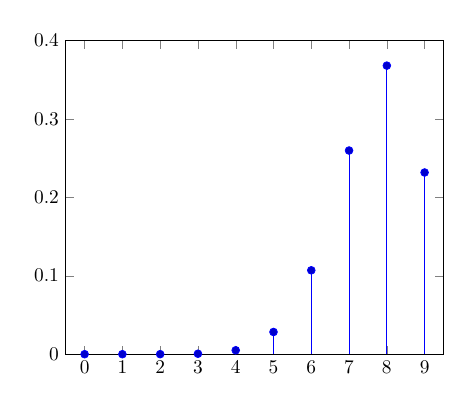
\begin{tikzpicture}[scale = 0.7]
\begin{axis} [ymin = 0, ymax = 0.4, xmin = -0.5, xmax = 9.5,
		y tick label style={
        /pgf/number format/.cd,
            fixed,
            precision=2,
        /tikz/.cd
    }, xtick = {0,1,2,3,4,5,6,7,8,9}]
\addplot+[ycomb] plot coordinates {(0, 0.00000003) (1, 0.000002) (2, 0.000045) (3, 0.00058) (4,0.005) (5, 0.0283) (6, 0.10692) (7,0.2596) (8,0.3678) (9,0.2316)}; 
\end{axis}
\end{tikzpicture}
\end{center}

\par
To derive this probability mass function, imagine recording of the results of the Bernoulli trials as an $n$ letter long string of $S$'s and $F$'s, representing success and failure respectively. We saw in Section \ref{sec 2.2} on combinations that the number of such strings in which $x$ successes occur is $\binom{n}{x}$.
\par
Consider any such string, say $SFSSSFF$. In this case $n=7$ and four successes occurred. The probability this sequence of outcomes occurs is not hard to calculate since we're performing independent Bernoulli trials, each with the same probability of success. Every $S$ occurs with probability $p$, and every $F$ with probability $1-p$. Since there are four $S$'s and three $F$'s, and the trials are independent, this string occurs with probability $p^4(1-p)^3$.
\par
In total then, there are $\binom{n}{x}$ sequences of outcomes with $x$ successes, and each sequence occurs with probability $p^x(1-p)^{n-x}$, so $P(X = x) = \binom{n}{x}p^x(1-p)^{n-x}$.
\par
The number of heads in $n$ flips of a coin is the example that should immediately come to mind when you think of a binomial distribution, but binomial distributions also appear in many practical contexts involving samples.

\begin{examp}Suppose that in a certain country's election, $56\%$ of the voting population will vote for a particular candidate, Bob. If you select seven members of the voting population uniformly at random, and ask them who they'll vote for (assume they'll answer honestly), what is the probability your poll will incorrectly conclude that Bob will not win a majority of the vote?
\par
\noindent Let $X$ represent the number of people who respond by saying that they'll vote for Bob. If we regard such a response as a success, and each interview is done without knowledge of the results of any of the others, then $X \sim Binomial(7, 0.56)$.
\par
\noindent The result we're seeking is the probability that there are fewer than four successes, which we calculate from the pmf as follows.
\eqns{P(X \leq 3) &= \sum_{i=0}^{3} P(X = i) = \sum_{i=0}^{3} \binom{7}{i}(0.56)^{i}(0.44)^{7-i} \\
&\simeq 0.0032 + 0.0284 + 0.1086 + 0.2304 \\
&= 0.3706 \simeq 37\%}
\par
\noindent There is a $37\%$ chance that the results of this poll will incorrectly predict that Bob will not win a majority of the vote.
\end{examp}
\par
\rmk It would be easier to use the cdf to evaluate $P(X \leq 3)$, but unfortunately, the cdf for a binomial distribution does not have a simple closed form, so we're stuck summing the values of the pmf.
\par
One of the reasons the binomial distribution appears in many contexts is that the process of evaluating a claim by doing repeated independent trials, which could be interviews, simulations, or literal laboratory experiments, is such a fundamental practice.
\par
When we get into statistics later in the course, we'll show that as our sample of results grows larger, the probability of an incorrect prediction shrinks, and shrinks at a fast enough rate that it's possible to draw a reasonably accurate conclusion without having to use an unrealistically large sample.

\begin{thm}\index{Binomial Distribution!expected value of}\index{Binomial Distribution!variance of}If $X \sim Binomial(n,p)$, then $E(X) = np$ and $\Var(X) = np(1-p)$.
\end{thm}
\begin{pf}
If $X$ is binomial with parameters $n$ and $p$, then $X$ is the number of successes in $n$ independent Bernoulli trials, which means $X = X_1 + X_2 + ... + X_n$, where each $X_i \sim Bernoulli(p)$. The expected value of each $X_i$ is $p$ by Theorem \ref{BernoulliExpectation}, so by linearity of expectation,
\eqns{E(X) &= E(X_1 + X_2 + ... + X_n) \\
&=E(X_1) + E(X_2) + ... + E(X_n) \\
&= p+p+ ... +p = np}
\par
\noindent The variance can be derived similarly with the aid of Corollary \ref{expectationandvarianceofindependentsum}.
\eqns{\Var(X) &= \Var(X_1 + X_2 + ... + X_n) \\
&=\Var(X_1) + \Var(X_2) + ... + \Var(X_n) \\
&= p(1-p)+p(1-p)+ ... +p(1-p) = np(1-p)}
\end{pf}
%\eqns{E(X^2) &= \sum_{x = 0}^{n} x^2 \binom{n}{x}p^x(1-p)^{n-x} = \sum_{x = 0}^{n} xn \binom{n-1}{x-1}p^x(1-p)^{n-x}  \\ &= np \sum_{x = 1}^{n} x\binom{n-1}{x-1}p^{x-1}(1-p)^{(n-1)-(x-1)} \\ &= np\sum_{y = 0}^{m} (y+1) \binom{m}{y}p^y(1-p)^{m-y} \text{\ \ where $y = x-1$ and $m = n-1$} \\
%&= np \left(\sum_{y = 0}^{m} y \binom{m}{y}p^y(1-p)^{m-y} + \sum_{y = 0}^{m} \binom{m}{y}p^y(1-p)^{m-y} \right) \\
%&= np \left(\sum_{y = 0}^{m} mp \binom{m-1}{y-1}p^{y-1}(1-p)^{(m-1)-(y-1)} + \sum_{y = 0}^{m} \binom{m}{y}p^y(1-p)^{m-y} \right) \\
%&= np \left(mp\sum_{y = 0}^{m} \binom{m-1}{y-1}p^{y-1}(1-p)^{(m-1)-(y-1)} + \sum_{y = 0}^{m} \binom{m}{y}p^y(1-p)^{m-y} \right) \\
%&=np (mp(p+(1-p))^{m-1}) + (p+(1-p))^m) \text{\ \ by the binomial theorem}\\
%&= np((n-1)p(1)^{m-1} + 1^{m})  = np((n-1)p + 1) = np^2(n-1)+np \\
%&= n^2p^2- np^2 + np = n^2p^2 +np(1-p)}
\par

\begin{examp} Let $X$ be the number of doubles in five rolls of a pair of dice, and let $Y$ be the number of heads in three flips of a fair coin. Which quantity is larger on average? Which quantity is more variable?
\par
\noindent $X$ is a binomial random variable with $n = 5$ and $p = \frac{6}{36} = \frac{1}{6}$, so $E(X) = np = \frac{5}{6}$ and $\Var(X) = np(1-p) = 5(\frac{1}{6})(\frac{5}{6}) = 25/36 \simeq 0.694$.
\par
\noindent $Y$ is a binomial random variable with $n = 3$ and $p = \frac{1}{2}$, so $E(Y) = np = \frac{3}{2}$ and $\Var(X) = np(1-p) = 3(\frac{1}{2})(\frac{1}{2}) = 3/4 \simeq 0.75$.
\par
\noindent Therefore, $Y$ is larger on average. The second question is somewhat ambiguous, but if we use the variance as our measure, $Y$ is a little more variable then $X$.
\end{examp}

\begin{examp}Edward lives in a country with very unreliable mail system. Only 7\% of parcels sent in the mail make it to their destination. He wants to send two \$20 books to his brother. If he sends them in one parcel, the postage is \$5.20, and if he sends them separately, the postage is \$3.30 for each book. To minimize the expected value of his expenses from a single attempt (loss + postage), which method is preferable?
\par
\noindent Let $X \sim Bernoulli(0.07)$, then sending both books in one parcel, the \$5.20 postage charge always applies, and \$40 is lost if $X = 1$. If $L$ represents Edward's loss, then $L = 5.20 + 40X$, and therefore $E(L) = 5.20 + 40E(X) = 5.20 + 40 \cdot 0.07 = 8$.
\par
\noindent On the other hand, if the two books are sent separately, then $L = 6.60 + 20Y$, where $Y \sim Binomial(2,0.07)$. Thus, $E(L) = 6.60 + 20E(Y) = 6.60 + 20 \cdot 2 \cdot 0.07 = 9.4$, so sending both books in one package is the better option.


\end{examp}

\section{The Geometric Distribution}\label{GeometricDist}

Binomial random variables result from performing independent Bernoulli trials a fixed number of times, and counting the number of successes. If instead, we repeat independent Bernoulli trials only until the first success occurs, and count the number of trials that were performed, we obtain a geometric random variable.

\begin{defn}\index{Geometric Distribution}\index{Distribution!Geometric}The random variable $X$ has a geometric distribution with parameter $p$, written $X \sim Geometric(p)$, if
\renewcommand*{\arraystretch}{1.35}
\eqns{f_X(x) = \left\{
\begin{array}{cl}
      (1-p)^{x-1}p & \text{ if \ } x = 1, 2, 3, ... \\
      0 & \text{ otherwise } \\ \end{array}.
\right.}
\renewcommand*{\arraystretch}{1}
\end{defn}

\par
\noindent On the left is the pmf of a geometric distribution with $p = 0.7$, and on the right is the pmf of a geometric distribution with $p=0.1$. Note that geometric random variables take arbitrarily large values, so both graphs continue to the right indefinitely, each approaching zero.

\begin{center}
\begin{tikzpicture}[scale = 0.7]
\begin{axis} [ymin = 0, ymax = 0.8, xmin = 0.01, xmax = 6.5,
		y tick label style={
        /pgf/number format/.cd,
            fixed,
            precision=2,
        /tikz/.cd
    }]
\addplot+[ycomb] plot coordinates {(1,0.7) (2,0.21) (3, 0.063) (4, 0.0189) (5, 0.00567) (6,0.0017)}; 
\end{axis}
\end{tikzpicture} \ \ \  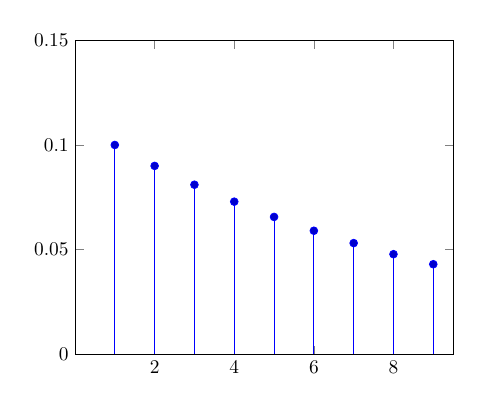
\begin{tikzpicture}[scale = 0.7]
\begin{axis} [ymin = 0, ymax = 0.15, xmin = 0.01, xmax = 9.5,
		y tick label style={
        /pgf/number format/.cd,
            fixed,
            precision=2,
        /tikz/.cd
    }]
\addplot+[ycomb] plot coordinates {(1,0.1) (2,0.09) (3,0.081) (4,0.0729) (5,0.06561) (6,0.059) (7,0.0531) (8,0.0478) (9,0.0430)}; 
\end{axis}
\end{tikzpicture}
\end{center}
\par
The derivation of the probability mass function can be done using the same ideas we used in the case of the binomial distribution. We can represent the outcomes of a sequence of repeated Bernoulli trials using $S$'s for success and $F$'s for failure. If we stop performing trials when the first success occurs, then the sequence of outcomes must be some number of $F$'s followed by an $S$.
\par
If the result was $FFFFFS$, then six trials were performed. Each failure occurs with probability $1-p$, each success with probability $p$, and the trials are independent, so the probability this sequence occurs is $(1-p)^5p$. The same argument generalizes to any sequence of $F$'s followed by an $S$ and hence the probability that $x$ trials must be performed before observing the first success is $(1-p)^{x-1}p$.
\par
\begin{examp}\label{GeoCards}Cards are repeatedly drawn with replacement from a shuffled deck. What is the probability that none of the first three cards that appear are face cards?
\par
\noindent If we define a success as drawing a face card, then the number of draws $X$ until the first face card appears has $X \sim Geometric(\frac{12}{52})$.
\par
\noindent
The probability that none of the first three cards is a face card is $P(X > 3)$, which we can calculate from the pmf.
\eqnsgap{P(X > 3) &= 1 - \sum_{x=1}^{3}P(X = x) = 1 - \frac{12}{52} - \frac{40}{52}\cdot\frac{12}{52} - \frac{40}{52}\cdot\frac{40}{52}\cdot\frac{12}{52} \simeq 0.455}
\end{examp}
\par
In this example we could have made efficient use of the cdf to quickly calculate this probability. Let's write down the cdf for a geometric random variable so we can do this in the future. The proof is left as an exercise.

\begin{prop}
If $X \sim Geometric(p)$, the cdf of $X$ is given by the expression below, where $\lfloor x \rfloor$ denotes the largest integer smaller than or equal to $x$.
\renewcommand*{\arraystretch}{1.35}
\eqns{F_X(x) = \left\{
\begin{array}{cl}
      1 - (1-p)^{\lfloor x \rfloor} & \text{ if \ } x \geq 1\\
    0 & \text{if \ } x < 1 \\ \end{array}
\right.}
\renewcommand*{\arraystretch}{1}
\end{prop}

%\begin{pf} Suppose that $x$ is a positive integer, then
%\eqns{P(X \leq x) = \sum_{k=0}^{x} P(X = k) = p + (1-p)p + (1-p)^2p + ... + (1-p)^{k-1}p.}
%\par
%\noindent If we multiply both sides by $1-p$, we obtain the expression
%\eqnspar{(1-p)P(X \leq x) &= (1-p)p + (1-p)^2p + (1-p)^3p +  ... + (1-p)^{k}p.}
%\par
%\noindent Notice that the right hand side is now missing the initial term, $p$, that was present above, and has an extra $(1-p)^kp$ term on the end. Therefore, we have
%\eqns{(1-p)P(X \leq x) &= P(X \leq x) - p + (1-p)^{k}p \\
%(1-p)P(X \leq x) - P(X \leq x) &= -p + (1-p)^kp \\
%-pP(X \leq x) &= -p + (1-p)^kp \\
%P(X \leq x) &= 1 - (1-p)^k.}
%\par
%\noindent If $x$ is not an integer, but is greater than 1, then $F_X(x) = F_X(\lfloor x \rfloor)$ since the random variable $X$ can take only positive integer values.
%\end{pf}

\par In Example \ref{GeoCards} above, $X \sim Geometric(\frac{12}{52})$, so $F_X(x) = 1 - (1-\frac{12}{52})^{x}$ for all integers $x > 1$. We could obtain the result in that example via
\eqnspar{P(X > 3) = 1 - P(X \leq 3) = 1 - F_X(3) =1 - \left( 1 - \left(1 - \left(\textstyle\frac{12}{52}\right)\right)^3\right) \simeq 0.455.}

\begin{thm}\label{GeometricExpectation}\index{Geometric Distribution!expected value of}\index{Geometric Distribution!variance of}
If $X \sim Geometric(p)$, then $E(X) = \frac{1}{p}$ and $\Var(X) = \frac{1-p}{p^2}$.
\end{thm}
\begin{pf} The expected value can be calculated with clever use of derivatives. From the definition of expected value and the pmf of $X$,
\eqns{E(X) &= \sum_{x =1}^{\infty} x f_X(x) = \sum_{x =1}^{\infty} x(1-p)^{x-1}p = p\sum_{x =1}^{\infty} x(1-p)^{x-1}.}
\par
\noindent Observe that $\frac{d}{dp}(1-p)^x = x(1-p)^{x-1}(-1)$ and hence $\frac{d}{dp}(1-p)^x(-1) = x(1-p)^{x-1}$, regarding $p$ as a variable and $x$ as a constant. We can therefore rewrite the sum as
\eqns{&p\, \sum_{x =1}^{\infty} \frac{d}{dp}(1-p)^{x}(-1) = -p \,\sum_{x=1}^{\infty} \frac{d}{dp}(1-p)^x \\  &\stackrel{!}{=}-p\, \frac{d}{dp} \left( \,\sum_{x=1}^{\infty} (1-p)^x\right) = -p\, \frac{d}{dp} \left(\frac{1-p}{1 - (1-p)}\right) \\ &= -p \,\frac{d}{dp}\left(\frac{1-p}{p}\right).}
\par
\noindent The infinite series was summed with the geometric series sum formula. To finish, we only need to evaluate the derivative using the quotient rule.
\eqns{E(X) = -p \, \frac{d}{dp} \left( \frac{1-p}{p} \right)= -p \, \frac{(-1)(p) - (1-p)(1)}{p^2} = -p \frac{-1}{p^2} = \frac{1}{p}}
\end{pf}

\par
We'll omit the argument for the variance. In fact, the same trick involving the derivative can be used twice to evaluate the infinite sum that defines $E[X^2]$, and we can obtain the variance with $\Var(X) = E[X^2] - (E[X])^2$.
\par
There is one step here that's suspect, the point where we factor the derivative out of the sum (marked with !). This works for finite sums, beacuse the sum rule in calculus tells us $\frac{d}{dp}(f(p) + g(p)) = \frac{d}{dp} f(p) + \frac{d}{dp} g(p)$. Does this same principle apply for infinite sums? Sometimes. The subtleties of this issue are beyond the scope of this course, but this instance turns out to be one where the move is justified.

\begin{examp} 
Consider a noisy communications channel. There is a $71\%$ chance that a message sent over this channel will become garbled and be unintelligible on the receiving end. Suppose that a message is sent until it's received intact without having become garbled, and each attempt takes 2 minutes. What is the probability the message will be correctly received in eight minutes or fewer? What is the average amount of time required before the message is received intact?
\par
\noindent If $X$ represents the number of attempts required to receive the message intact, then $X \sim Geometric(0.29)$, since there is an $29\%$ chance of a successful transmission, and $Y = 2X$ is the amount of time required to receive the message intact. We can then easily calculate $P(Y \leq 8)$ and $E(Y)$ from the results in this section.
\eqnspar{P(Y \leq 8) &= P(X \leq 4) & E(Y) &= E(2X) \\
&= 1 - (1-0.29)^4 & &= 2E(X) \\
&\simeq 1 - 0.254 = 0.746 & &=2 \cdot \textstyle\frac{1}{0.29}  \simeq 6.90}
\par
\noindent Thus, there is a $74.6\%$ chance the message will be correctly received in eight minutes or less, and the average amount of time required is $6.90$ minutes.
\end{examp}

\par
Notice that the formula $E(X) = 1/p$ has a remarkably intuitive interpretation. If one in every five people in a certain group drives a red car, then how many people from this group would you have to meet, on average, to find one who drives a red car? Five, right? In fact, that's precisely correct, since if $X \sim Geometric(\frac{1}{5})$, then $E(X) = 1/\frac{1}{5}=5$.
\par
In the concluding sections of this chapter, we've studied the Uniform, Bernoulli, Binomial, and Geometric distributions. If you look through a few probability texts, you might encounter the Poisson, Hypergeometric, and Negative Binomial distributions as well, but we can't cover everything, so we'll leave these out of our discussion.




